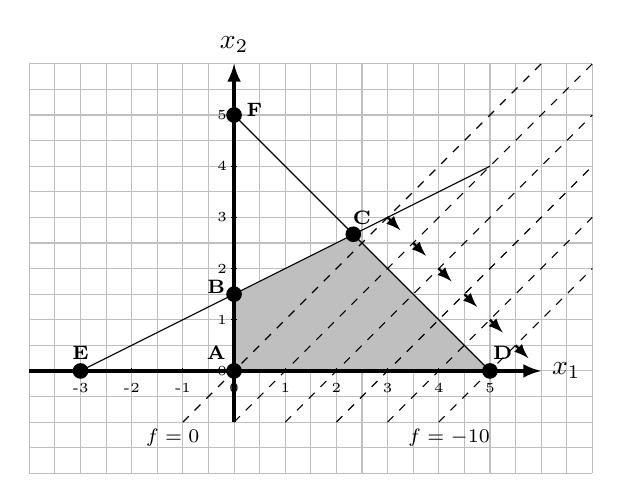
\begin{tikzpicture}[scale=0.65]
  \fill[gray!50] (0, 0) -- (0, 1.5) -- (7/3, 8/3) -- (5, 0) -- cycle;  
  \draw[gray!50, thin, step=0.5] (-4, -2) grid (7, 6);
  \draw[very thick, -latex] (-4, 0) coordinate(x1) -- (6, 0) coordinate(x2) node[right] {$x_1$};
  \draw[very thick, -latex] (0, -1) coordinate(y1) -- (0, 6) coordinate(y2) node[above] {$x_2$};
  \foreach \x in {-3, ..., 5} {
    \draw (\x, 0.05) -- (\x, -0.05) node[below] {\tiny\x};
  }
  \foreach \y in {0, ..., 5} {
    \draw (-0.05, \y) -- (0.05, \y) node[left] {\tiny\y};
  }
  \draw (0, 5) coordinate (a1) -- node[above left, sloped] {} (5, 0) coordinate (a2) ;
  \draw (-3, 0) coordinate (b1) -- node[above right, sloped] {} (5, 4) coordinate (b2);	
  \draw[dashed] (-1, -1) -- (6, 6);
  \draw[dashed] (0, -1) -- (7, 6);
  \draw[dashed] (1, -1) -- (7, 5);
  \draw[dashed] (2, -1) -- (7, 4);
  \draw[dashed] (3, -1) -- (7, 3);
  \draw[dashed] (4, -1) -- (7, 2);
  \node at (0, 0) [circle, fill, inner sep=2pt] {};
  \node at (0, 1.5) [circle, fill, inner sep=2pt] {};
  \node at (0, 5) [circle, fill, inner sep=2pt] {};
  \node at (-3, 0) [circle, fill, inner sep=2pt] {};
  \node at (2.33, 2.67) [circle, fill, inner sep=2pt] {};
  \node at (5, 0) [circle, fill, inner sep=2pt] {};
  \node at (-0.35, 0.35) {\scriptsize{\textbf{A}}};
  \node at (-0.35, 1.65) {\scriptsize{\textbf{B}}};
  \node at (2.5, 3) {\scriptsize{\textbf{C}}};
  \node at (5.25, 0.35) {\scriptsize{\textbf{D}}};
  \node at (-3, 0.35) {\scriptsize{\textbf{E}}};
  \node at (0.4, 5.1) {\scriptsize{\textbf{F}}};
  \node at (-1.2, -1.3) {\scriptsize{$f=0$}};
  \node at (4.2, -1.3) {\scriptsize{$f=-10$}};
  \draw[-latex, thick] (3, 3) -- (3.25, 2.75);
  \draw[-latex, thick] (3.5, 2.5) -- (3.75, 2.25);
  \draw[-latex, thick] (4.0, 2.0) -- (4.25, 1.75);
  \draw[-latex, thick] (4.5, 1.5) -- (4.75, 1.25);
  \draw[-latex, thick] (5.0, 1.0) -- (5.25, 0.75);
  \draw[-latex, thick] (5.5, 0.5) -- (5.75, 0.25);
\end{tikzpicture}

